Our Smart Fridge uses two devices, an ESP32 microcontroller and a Raspberry Pi (RPi), to perform all its local features.
The ESP32 talks to all the sensors of the refrigerator.
The RPi receives data from the microcontroller, process it and then send data to server through the internet.
Multiple sensors are connected to the microcontroller, an OV2640 camera module, a HAL effect switches, and a weight sensor.
An over view of this can be seen in Figure \ref{fig:block_diagram}.

The HAL effect switch senses when the fridge is open and closed, 
this is used to inform when to use the camera to capture incoming items and also to remind the user to close the door if left open using a simple buzzer.

The weight sensor inside the fridge detects the weight of each object placed in the refrigerator.
This sensor connects to the ESP32 through an ADC module that amplifies and produces more accurate measurements from the load cell.

Images from the camera module will be captured by the ESP32, only when the door is open, and sent to the RPi.

The RPi uses OpenCV to process the image and retrieve the barcode data, as well as if the item is entering of leaving the fridge.
Other machine vision software, possible using machine learning, will also be employed to object where the barcode cannot be scanned.

Once a barcode has been captured, or an item has been identified, 
information about that item and data such as weight, expiry date, etc, will be sent to a PostgreSQL server using our REST API.
The server then keeps track of what transfers in and out of the fridge.
Alerts will be sent to the user when an object in the fridge is closer to its expiration date as well as occasional recommendations for recipes. 
The website and app will allow the user to keep track of the inventory,
as well as manually edit the inventory in case the fridge misses items.
The website or app requests data from the server to be up to date with the contents inside the refrigerator.

\begin{figure}[H]        
    \centering
    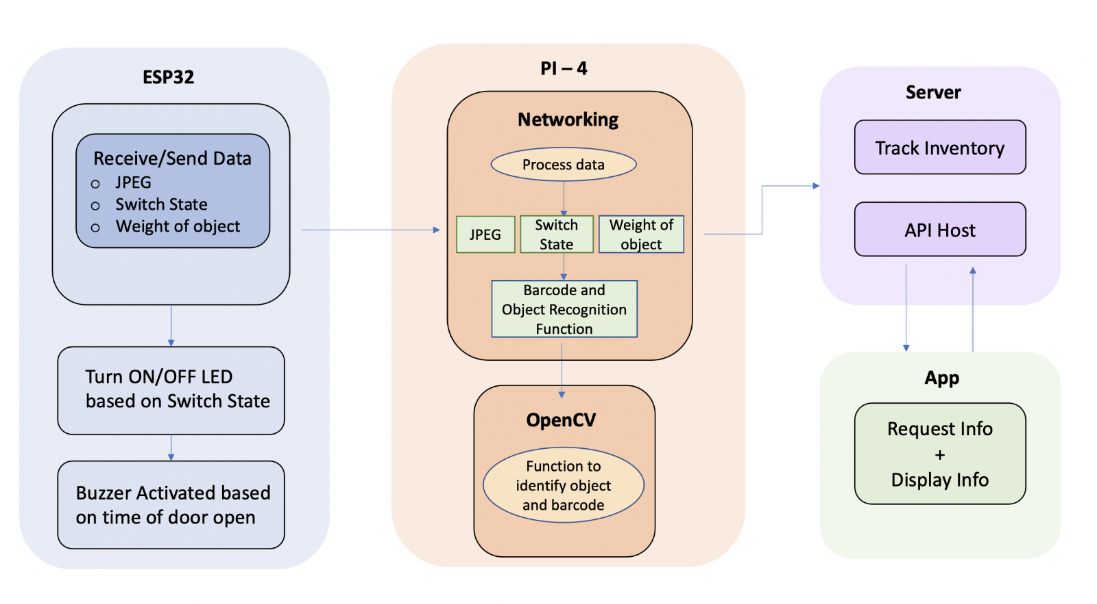
\includegraphics[width=0.5\textwidth]{block-diagram.png}
    \caption{Block Diagram}
    \label{fig:block_diagram}
\end{figure} 
